\subsection{感知机}
\label{sec:classification-perceptron}

Fisher先估计类统计量再决定投影方向。若任务只要求给出类别，也可以直接用预测错误调整边界。例如两类点虽然可以被一条直线分开，却沿不同方向伸展，不适合共享协方差的描述；寻找分隔线仍是有意义的任务，并不需要先把每类的分布拟合好。

\term{感知机}（perceptron）从一组初始权重出发，逐个检查训练样本；遇到分类条件被违反的样本，就沿提高其正确类别得分的方向修正权重。这样，标签直接告诉算法边界需要怎样移动。算法可在任意训练集上运行；若训练集具有正间隔可分性，才有后面证明的有限更新保证。Rosenblatt在1958年的论文中研究了这一学习机制，本节介绍其中广泛使用的线性阈值模型与误差修正规则\scite{rosenblatt1958}。

\subsubsection{模型结构}
\label{sec:classification-perceptron-model}

本小节先使用二分类标签$y_i\in\{-1,+1\}$。为了使偏置在更新规则和收敛证明中始终处于同一坐标系，引入\term{增广向量}（augmented vector），即在输入末尾补一个恒为$1$的分量，并把偏置并入参数：
\begin{equation}
  \label{eq:classification-perceptron-augmented}
  \tilde{\bm{x}}=
    \begin{pmatrix}\bm{x}\\1\end{pmatrix},\qquad
  \tilde{\bm{w}}=
    \begin{pmatrix}\bm{w}\\b\end{pmatrix}
    \in\mathbb{R}^{d+1}.
\end{equation}
其中$\bm{w}\in\mathbb{R}^{d}$，$b\in\mathbb{R}$。分类规则为
\begin{equation}
  \label{eq:classification-perceptron-prediction}
  f(\bm{x})=\operatorname{sign}
    (\tilde{\bm{w}}^{\top}\tilde{\bm{x}})
    =\operatorname{sign}(\bm{w}^{\top}\bm{x}+b).
\end{equation}
约定$\operatorname{sign}(s)=+1$当$s\geq0$，否则为$-1$。非退化边界$\bm{w}^{\top}\bm{x}+b=0$是在$d$维输入空间中的$(d-1)$维超平面。它与二分类LDA具有相同的边界形式；这里的参数来自错误反馈，输出是类别得分与标签，概率需要另建模型。

线性表示的边界也很具体。例如异或任务把$(0,0)$、$(1,1)$标为负类，把$(1,0)$、$(0,1)$标为正类。按上述平局规则，前两点要求$b<0$和$w_1+w_2+b<0$，后两点要求$w_1+b\geq0$和$w_2+b\geq0$。前两式相加与后两式相加，对同一个$w_1+w_2+2b$给出矛盾要求。Minsky与Papert在1969年的《Perceptrons》中系统研究了此类表示能力限制；改变输入特征或加入非线性隐藏层可以越过单个线性边界的限制，但那已经改变了模型族\scite{minsky1969}。

\subsubsection{参数学习}
\label{sec:classification-perceptron-learning}

从$\tilde{\bm{w}}^{(0)}=\bm{0}$出发，若当前样本满足$y_i\langle\tilde{\bm{w}}^{(t)},\tilde{\bm{x}}_i\rangle\leq0$，便进行一次更新：
\begin{equation}
  \label{eq:classification-perceptron-update}
  \tilde{\bm{w}}^{(t+1)}
    =\tilde{\bm{w}}^{(t)}+\eta y_i\tilde{\bm{x}}_i,
  \qquad \eta>0 .
\end{equation}
这里$t$只数实际更新，学习率$\eta$保持不变。拆开最后一个分量，就是$\bm{w}\leftarrow\bm{w}+\eta y_i\bm{x}_i$和$b\leftarrow b+\eta y_i$。同一个样本的有符号得分增加$\eta\|\tilde{\bm{x}}_i\|_2^2$，所以更新确实朝修正当前判断的方向移动；但它可能同时破坏其他样本的正确分类，因而需要反复遍历。零得分也触发更新，即使按平局规则恰好预测为正确的正类，仍要求它离开边界。

图~\ref{fig:classification-perceptron-update}把这一步写成具体数值。取当前参数$\bm w=(1,0)^{\top}$、$b=-1$，正类点$\bm x_i=(0.5,1)^{\top}$的得分为$-0.5$，触发更新。学习率为$0.5$时，权重变为$(1.25,0.5)^{\top}$，偏置变为$-0.5$，当前点的得分增加到$0.625$。图中边界因此同时改变位置和方向；判断是否继续更新，仍要逐个检查后续样本。

\begin{figure}[htbp]
  \centering
  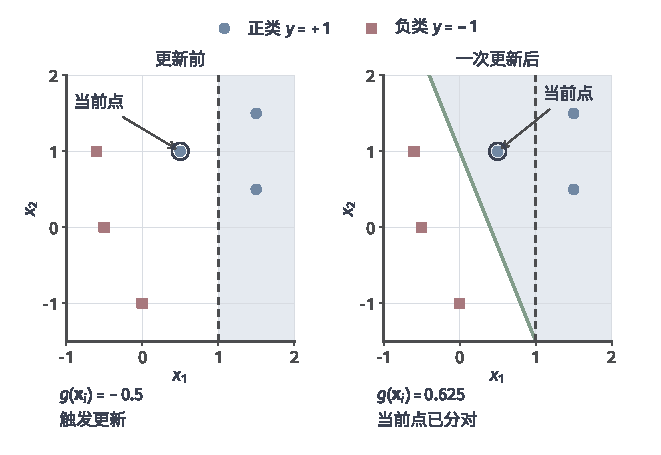
\includegraphics[width=112.000mm]{figures/04-classic-models/00-shared/matplotlib/classification-perceptron-update/figure.pdf}
  \caption{错分正类点触发的一次感知机更新。六个点为教学构造，坐标无量纲，两面板共用坐标范围；蓝圆、红方分别为正负类，黑色圆环标出当前点。浅蓝区域为正类预测区域，虚线为旧边界$x_1=1$，绿色实线为新边界$1.25x_1+0.5x_2=0.5$。偏置随权重一起更新，当前点由负得分变为正得分。}
  \label{fig:classification-perceptron-update}
\end{figure}

\begin{algorithm}[带遍历上限的感知机训练]
  \label{alg:classification-perceptron}
  \begin{algorithmic}[1]
    \Require $D_n$，固定学习率$\eta>0$，最大遍历轮数$E\geq1$
    \Ensure 参数$\tilde{\bm{w}}$与是否已验证收敛的状态
    \State $\tilde{\bm{w}}\gets\bm{0}$
    \For{$e=1,\ldots,E$}
      \State $m\gets0$
      \For{$i=1,\ldots,n$}
        \State $\tilde{\bm{x}}_i\gets(\bm{x}_i^{\top},1)^{\top}$
        \If{$y_i\langle\tilde{\bm{w}},\tilde{\bm{x}}_i\rangle\leq0$}
          \State $\tilde{\bm{w}}\gets\tilde{\bm{w}}+\eta y_i\tilde{\bm{x}}_i$
          \State $m\gets m+1$
        \EndIf
      \EndFor
      \If{$m=0$}
        \State \Return $(\tilde{\bm{w}},\text{已收敛})$
      \EndIf
    \EndFor
    \State \Return $(\tilde{\bm{w}},\text{达到轮数上限})$
  \end{algorithmic}
\end{algorithm}

一整轮没有更新时，所有样本都是在同一个参数下得到严格正的有符号得分，才构成收敛证据。达到轮数上限时返回的是预算内的当前解，可分性仍未由这一停止状态判定。稠密实现每轮需要$O(nd)$运算，除训练集外只需$O(d)$参数空间；样本访问顺序可以改变输出的分隔面。

从优化角度看，定义\term{感知机损失}（perceptron loss）
\begin{equation}
  \label{eq:classification-perceptron-loss}
  \ell_{\mathrm{P}}(\tilde{\bm{w}};\bm{x}_i,y_i)
    =\max\{0,-y_i\langle\tilde{\bm{w}},\tilde{\bm{x}}_i\rangle\}.
\end{equation}
为了把这项损失用于更新，先看它的两段：当带符号得分为负时，对参数求导得到$-y_i\tilde{\bm{x}}_i$；得分为正时，损失恒为零，梯度也是$\bm 0$。两段在零得分处相接，却给出不同斜率，普通梯度在这里没有定义。由于损失仍是凸的，可以使用次梯度；在交点处选择$-y_i\tilde{\bm{x}}_i$，仍满足支撑损失的仿射下界条件，也就得到式~\eqref{eq:classification-perceptron-update}。相应的凸优化工具可参考\BookChapterRef{chap:optimization}{卷一《数学准备：计算、分析与几何》的“最优化”章}。

上述更新逐样本执行；随机抽取样本时才相应成为随机次梯度下降。这里使用的是零间隔损失，不是标准的\term{合页损失}（hinge loss）$\max\{0,1-y_i\langle\tilde{\bm{w}},\tilde{\bm{x}}_i\rangle\}$：合页损失要求正确侧得分不仅为正、还要高出1，达到1以后不再受罚，不足1时按缺口线性加价。前者在零参数处就对所有样本取零，因此“感知机损失为零”本身不能证明分类正确；算法在零得分处仍更新的约定不可省略。

\subsubsection{理论分析}
\label{sec:classification-perceptron-analysis}

在证明“更新会停止”之前，先要把“可分”这个条件说得更精确。仅仅“存在一条直线能分开”还不足以给出与数据无关的统一结论，因为直线可以无限贴近某些点；我们还要求存在一条分隔线，让所有样本到它的距离都不小于某个正数$\gamma$。这个$\gamma$称为\term{间隔}（margin），它衡量两类之间留了多宽的一条“空白走廊”。在这一表示下，正间隔可分是指存在单位向量$\bm{u}^\ast\in\mathbb{R}^{d+1}$和$\gamma>0$，使
\begin{equation}
  \label{eq:classification-perceptron-margin}
  \begin{aligned}
    y_i\langle\bm{u}^\ast,\tilde{\bm{x}}_i\rangle
      &\geq\gamma,\qquad i=1,\ldots,n,\\
    \|\bm{u}^\ast\|_2&=1,\qquad
    \|\tilde{\bm{x}}_i\|_2\leq R .
  \end{aligned}
\end{equation}
这里$R$约束的是增广输入，因此$R\geq\max_i\sqrt{\|\bm{x}_i\|_2^2+1}$。$\gamma$也是增广空间中的间隔；若$\bm{u}^\ast=(\bm{v}^{\top},a)^{\top}/\sqrt{\|\bm{v}\|_2^2+a^2}$，其分母包含偏置$a$，不同于原输入空间中以$\|\bm{v}\|_2$归一化的几何距离。有限训练集只要能被仿射超平面严格分开，就存在这样的正$\gamma$。

每次修正可能破坏已有判断，为什么这些修正不会无穷持续？关键是存在一个始终把所有样本分对的参考方向：更新朝该方向取得线性累积的进展，而参数范数的平方只能线性增长。Novikoff在1962年报告的证明清楚展示了这两个增长速度之间的矛盾\scite{novikoff1962}。

\begin{theorem}[感知机在有界可分样本下的最大更新次数]
  \label{thm:classification-perceptron-mistakes}
  若$D_n$满足式~\eqref{eq:classification-perceptron-margin}，从零参数出发，以固定$\eta>0$按式~\eqref{eq:classification-perceptron-update}更新，则对任意样本访问顺序，错误更新次数$M$满足
  \[
    M\leq\left(\frac R\gamma\right)^2 .
  \]
  这里错误更新包括零得分时的更新。若持续完整遍历训练集，且不因预算提前退出，算法在有限轮后得到所有训练样本上有符号得分均严格为正的参数。
\end{theorem}

\begin{proof}
  设第$t+1$次更新使用样本$i_t$。沿单位参考方向$\bm{u}^\ast$考察更新，得到
  \begin{align*}
    \langle\tilde{\bm{w}}^{(t+1)},\bm{u}^\ast\rangle
      &=\langle\tilde{\bm{w}}^{(t)},\bm{u}^\ast\rangle
        +\eta y_{i_t}\langle\tilde{\bm{x}}_{i_t},\bm{u}^\ast\rangle\\
      &\geq\langle\tilde{\bm{w}}^{(t)},\bm{u}^\ast\rangle+\eta\gamma .
  \end{align*}
  从零参数累加$M$次，便有
  \[
    \langle\tilde{\bm{w}}^{(M)},\bm{u}^\ast\rangle
      \geq M\eta\gamma .
  \]
  另一方面，展开更新后的平方范数：
  \begin{align*}
    \|\tilde{\bm{w}}^{(t+1)}\|_2^2
      &=\|\tilde{\bm{w}}^{(t)}\|_2^2
        +2\eta y_{i_t}
          \langle\tilde{\bm{w}}^{(t)},\tilde{\bm{x}}_{i_t}\rangle\\
      &\quad+\eta^2\|\tilde{\bm{x}}_{i_t}\|_2^2\\
      &\leq\|\tilde{\bm{w}}^{(t)}\|_2^2+\eta^2R^2 .
  \end{align*}
  不等式使用了更新条件：交叉项非正；并使用同一增广空间中的长度界$R$。再次累加，得到$\|\tilde{\bm{w}}^{(M)}\|_2^2\leq M\eta^2R^2$。由Cauchy--Schwarz不等式和$\|\bm{u}^\ast\|_2=1$，
  \[
    M\eta\gamma
      \leq\langle\tilde{\bm{w}}^{(M)},\bm{u}^\ast\rangle
      \leq\|\tilde{\bm{w}}^{(M)}\|_2
      \leq\eta R\sqrt{M}.
  \]
  $M=0$时结论直接成立；$M>0$时除以$\eta\sqrt M$再平方，得到所述界。因此更新不可能无限发生。持续完整遍历会在最后一次更新之后再检查所有样本；若仍有非正得分就还会更新，产生矛盾，故最终必有一整轮没有更新。
\end{proof}

这个界不显式含$n$，也不依赖访问顺序，但$R$和$\gamma$随数据而定；增加样本可能缩小可分间隔。它只约束更新次数，不包括寻找错误时检查正确样本的开销。对于算法~\ref{alg:classification-perceptron}的逐轮扫描，若不提前截断，至多需要$M+1$轮，包括最终的无更新确认轮。

若数据不可分，有限更新保证失效，持续遍历可能反复更新，此时可以限制训练预算并保留历史较好解，或采用允许间隔违约的在线方法。这些处理改变了停止或选解方式，仍须分别分析。有限更新结论说明训练程序何时停止，不直接给出新样本错误率。尤其不可分、带噪声或预算提前结束时，应按实际返回的参数在独立数据上评价；不能把当前训练集的可分性当作未来样本也可分的证据。

\subsubsection{核感知机：改变输入表示}
\label{sec:classification-perceptron-kernel}

若问题在于原空间不能线性分开，可把输入换成特征映射$\bm{\phi}(\bm{x})$。核函数$K(\bm{x},\bm{z})=\langle\bm{\phi}(\bm{x}),\bm{\phi}(\bm{z})\rangle$直接计算映射后的内积，省去显式构造高维坐标，得到\term{核感知机}（kernel perceptron）。为与前文偏置一致，使用增广映射$(\bm{\phi}(\bm{x}),1)$及其核$\tilde K(\bm{x},\bm{z})=K(\bm{x},\bm{z})+1$。零初始化、单位学习率下，参数在特征空间中是更新样本的线性组合，预测可写为
\begin{equation}
  \label{eq:classification-kernel-perceptron}
  f(\bm{x})=\operatorname{sign}
    \left(\sum_{i=1}^{n}\alpha_i y_i
      [K(\bm{x}_i,\bm{x})+1]\right).
\end{equation}
这里$\alpha_i$是样本$i$的更新次数；遇到非正有符号得分时令$\alpha_i\leftarrow\alpha_i+1$。必须选用正定核，即它在任意有限输入集上生成半正定Gram矩阵，才能作上述内积解释；有限更新还要求增广特征空间内存在正间隔，长度界相应变为$\sqrt{K(\bm{x}_i,\bm{x}_i)+1}$的上界。预测需要访问系数非零的样本，数量可能随训练增长。将内积推广到特征空间的思路可追溯至Aizerman、Braverman与Rozonoer在1964年的势函数研究\scite{aizerman1964}。

核与输入尺度共同决定映射后是否可分；预测成本则由需要保存的更新样本数决定。核化改变表示，不替代对标签噪声、停止规则和样本外误差的检查。

\subsubsection{投票与平均感知机：汇总历史状态}
\label{sec:classification-perceptron-voted}

最后一个参数状态可能对样本顺序敏感，可以汇总训练过程中的多个状态。Freund与Schapire在1999年研究的\term{投票感知机}（voted perceptron）保存历次权重，并按各状态持续使用的次数加权投票；同一论文也比较了用历史得分平均代替投票的方式\scite{freund1999}。

\paragraph{历史状态投票}
沿用本节的增广表示，设保存的状态为$\tilde{\bm w}_1,\ldots,\tilde{\bm w}_K$，$c_k>0$是第$k$个状态的计数，则投票预测为
\begin{equation}
  f_{\mathrm V}(\bm x)
  =\operatorname{sign}\!\left[
    \sum_{k=1}^{K}c_k\operatorname{sign}
      (\tilde{\bm w}_k^\top\tilde{\bm x})\right].
  \label{eq:classification-voted-perceptron}
\end{equation}
计数必须与更新同步。初始零参数的计数取零；本次检查未触发更新时，将当前状态的计数加一；触发更新时，保存新参数并把新状态的计数置为一，不再给被替换的旧状态加一。这里沿用非正有符号得分触发更新的约定，最后忽略计数为零的状态。计数取决于访问顺序与训练预算，并不是对新样本准确率的独立测量。保存与预测$K$个稠密状态均需考虑$O(Kd)$的代价。

\paragraph{平均参数预测}
\term{平均感知机}（averaged perceptron）改为先把这些增广参数平均：
\[
  \bar{\bm w}=\frac{\sum_{k=1}^{K}c_k\tilde{\bm w}_k}
                        {\sum_{k=1}^{K}c_k},
  \qquad
  f_{\mathrm A}(\bm x)=\operatorname{sign}
                    (\bar{\bm w}^\top\tilde{\bm x}).
\]
线性实现可在训练时累计参数和，最终只保存一组参数，额外存储与单次预测均为$O(d)$。投票先对每个得分取符号，再汇总标签；参数平均先汇总实值得分，再取符号，二者一般不同。前者的最终规则可以组合多个半空间判断，后者仍返回单个仿射得分；它们都改变训练结束后的输出方式，不能仅凭“汇总历史”判断哪种更适合任务。

\subsubsection{Pocket：保存预算内的较优结果}
\label{sec:classification-pocket}

不可分数据可能使参数反复改变，预算结束时的权重未必是已经检查过的最好结果。\term{口袋算法}（Pocket algorithm）通过保存历史参数处理这个问题。常用版本额外保存$\tilde{\bm{w}}_{\mathrm{pocket}}$：每次检查候选参数时，计算全训练集零一错误数，仅在严格改进时替换记录；预算用尽后返回记录参数。它适用于噪声或矛盾标签数据，返回预算内已检查候选中的最小训练错误解；每次候选比较还需要评估全训练集。Gallant在1990年的论文中系统讨论了Pocket及相关学习方法\scite{gallant1990}。

Pocket只改变返回哪组历史参数，候选得分仍是原坐标中的仿射函数。它需要额外评估全部训练样本，也不能消除前面异或任务的表示限制。这里改善的是有限预算下的返回规则，并未使不可分数据上的原更新停止，也不保证找到所有仿射分类器中的最小训练错误解。

\subsubsection{结构化感知机：联合决定多个标签}
\label{sec:classification-structured-perceptron}

如果任务是给一句话中的每个词标注词性，输出就从一个类别变成了一整条标签序列。逐词独立判类无法在同一个得分中评价相邻标签的组合；我们希望同时比较不同候选序列，并在预测错误时调整整条序列用到的特征。\term{结构化感知机}（structured perceptron）把多分类的得分比较推广到结构之间，用联合特征（joint feature）$\bm{\phi}(\bm{x},y)$描述输入与候选结构，预测
\[
  \hat y_i=\argmax_{y\in Y(\bm{x}_i)}
    \langle\bm{\theta},\bm{\phi}(\bm{x}_i,y)\rangle ,
\]
其中$Y(\bm{x}_i)$是候选结构集合，$\bm{\theta}$是与联合特征同维的参数。在这个集合中寻找当前得分最高的结构，称为解码（decoding）。解码错误时进行
\[
  \bm{\theta}\leftarrow\bm{\theta}
    +\eta\bigl[\bm{\phi}(\bm{x}_i,y_i)
      -\bm{\phi}(\bm{x}_i,\hat y_i)\bigr].
\]
要在同一输入上区分不同候选结构，联合特征中需要有随候选结构变化的分量。

考虑一个只说明机制的教学构造：固定两词输入“学习 方法”，只比较标签序列$(\text{动词},\text{名词})$与$(\text{名词},\text{名词})$。取两个联合特征，第一项记录“学习”被标为动词的次数，第二项记录相邻标签“动词$\to$名词”的次数；于是前一候选的特征向量为$(1,1)^\top$，后一候选为$(0,0)^\top$。若真实序列是前者、模型却选了后者，差值更新就给这两个参数各增加$\eta$，使正确候选相对于错误候选的得分增加$2\eta$。实际任务会记录更多词与标签的对应及标签转移特征；这里抽出两项，是为了看清相邻标签关系怎样进入同一个得分和同一次更新。这个小候选集可以直接枚举；序列很长时，候选数量会增长，能否高效寻找最高分结构还取决于联合得分是否具有可利用的分解。

联合特征决定哪些结构差异能够进入比较。若同一输入上的两个候选结构具有完全相同的$\bm\phi(\bm x,y)$，它们对所有参数都同分，候选得分无法区分两者，只能由固定的平局规则选择其中一个。词性标注中的相邻标签关系或更远处的依赖，因而需要由相应的特征记录；解码搜索再精确，也不能恢复特征没有保留的差异。需要的类别或结构偏置也作为联合特征中的相应指示分量处理；对所有候选都相同的常数项会在得分差中消去。结构化输出增加了解码成本，近似解码还可能改变哪些样本触发更新，需要与特征设计一同评价。Collins在2002年将这种更新与参数平均用于序列标注，提供了词性标注和短语识别等实例，也为比较感知机与条件随机场等结构化模型提供了参照\scite{collins2002}。这里只建立联合特征、解码与特征差更新的关系，完整结构化任务及高效序列解码留给后续对应任务卷。
